% \documentclass{article}
% %\usepackage[english]{babel}%
% \usepackage{graphicx}
% \usepackage{tabulary}
% \usepackage{tabularx}
% \usepackage[normalem]{ulem}
% \usepackage{cancel}
% \usepackage{tikz} 
% \usepackage{pdflscape}
% \usepackage{colortbl}
% \usepackage{lastpage}
% \usepackage{multirow}
% \usepackage{enumerate}
% \usepackage[shortlabels]{enumitem}
% \usepackage{color,soul}
% \usepackage{pdflscape}
% \usepackage{hyperref}
% %\usepackage[table]{xcolor}
% \usepackage{rotating}
% \usepackage{amsmath}
% \usepackage{fixltx2e}
% \usepackage{framed}
% \usepackage{mdframed}
% \usepackage[T1]{fontenc}
% \usepackage[utf8]{inputenc}
% \usepackage{textcomp}
% \usepackage{siunitx}
% \usepackage{ifthen}
% \usepackage{fancyhdr}
% \usepackage{gensymb}
% \usepackage{newunicodechar}
% \usepackage[document]{ragged2e}
% \usepackage[margin=1in,top=1.1in,headheight=57pt,headsep=0.1in]
% {geometry}
% \usepackage{ifthen}
% \usepackage{fancyhdr}
% \everymath{\displaystyle}
% \usepackage[document]{ragged2e}
% \usepackage{fancyhdr}
% \everymath{\displaystyle}
% \usepackage{empheq}

% \usepackage[most]{tcolorbox}

% \usepackage{booktabs} % Required for nicer horizontal rules in tables


% \usepackage{enumitem}

% %\usepackage[table,xcdraw]{xcolor}
% \usetikzlibrary{arrows}
% \linespread{2}%controls the spacing between lines. Bigger fractions means crowded lines%
% %\pagestyle{fancy}
% %\usepackage[margin=1 in, top=1in, includefoot]{geometry}
% %\everymath{\displaystyle}
% \linespread{1.3}%controls the spacing between lines. Bigger fractions means crowded lines%
% %\pagestyle{fancy}
% \pagestyle{fancy}
% \setlength{\headheight}{56.2pt}

% \definecolor{myblue}{rgb}{.8, .8, 1}
% \newcommand*\mybluebox[1]{%
% \colorbox{myblue}{\hspace{1em}#1\hspace{1em}}}

% \chead{\ifthenelse{\value{page}=1}{
\includegraphics[scale=0.3]{SCC}\\ \textbf \textbf Wastewater Constituents Analysis \& Laboratory Methods}}
% \rhead{\ifthenelse{\value{page}=1}{}{}}
% \lhead{\ifthenelse{\value{page}=1}{}{Wastewater Constituents Analysis \& Laboratory Methods}}
% \rfoot{\ifthenelse{\value{page}=1}{Module 1: WATR 048 - Spring 2019}{Module 1: WATR 048 - Spring 2019}}

% \lfoot{Shabbir Basrai}
% \cfoot{Page \thepage\ of \pageref{LastPage}}
% \renewcommand{\headrulewidth}{2pt}
% \renewcommand{\footrulewidth}{1pt}
% \begin{document}
% %\begin{empheq}[box=\mybluebox]{align}
% %a&=b\\
% %E&=mc^2 + \int_a^a x\, dx
% %\end{empheq}

% \newlist{steps}{enumerate}{1} % Defines "Steps" for enumerate as Step 1, Step 2 etc.
% \setlist[steps, 1]{label = Step \arabic*:} % Defines "Steps" for enumerate as Step 1, Step 2 etc.

% \setlist{nolistsep} % Reduce spacing between bullet points and numbered lists


%_______________________________________________________________________________________________________________________________________%
\chapterimage{Week5Ponds.jpg} % Chapter heading image

\chapter{Stabilzation Ponds}
% Chapter heading image

\begin{itemize}
\item Stabilization ponds and lagoons are bodies of water which treat wastewater using mainly natural processes including sunlight, algae and microorganisms for treating wastewater\\
\item While ponds are shallow and man-made, lagoons are bodies of water confined within natural boundaries.\\
\end{itemize}


\section{Advantages of ponds}\index{Advantages of ponds}	

\begin{itemize}	
\item Cheap to build and operate
\item Low maintenance and electrical costs
\item Do not require highly trained operational personnel
\item Provide treatment that can be equal to some secondary treatment processes and have fewer sludge handling issues.\\
\end{itemize}


\section{Disadvantages of ponds}\index{Disadvantages of ponds}	
\begin{itemize}	
\item Land intensive
\item Effluent quality varies with seasonal temperature changes
\item Suspended solids levels that can create regulatory problems.
\item System upsets almost always result in odor problems and recovery times may be weeks or months.
\item Not appropriate for colder climates
\end{itemize} 

\section{Types of Ponds}\index{Types of Ponds}	

\subsection{Anaerobic Ponds}\index{Anaerobic Ponds}	

\begin{itemize}	
\item Typically for treating raw sewage
\item Designed for BOD removal
\item 10-14 feet deep. 
\item High strength wastewater may be treated
\item Utilize anaerobic bacteria to break down the organic waste. 
\item Septic conditions in the lagoon and odors associated with septic sewer gases particularly hydrogen sulfide and its rotten egg odor. 
\item Most of the decomposition is accomplished by acid forming bacteria. 
\item The pH in these lagoons is usually below 6.5. 
\item They are total retention and do not have an effluent discharge. 
\item The anaerobic pond must be de-sludged approximately once every 2 to 5 years
\item Organic loading of 200-1000 lbs. $BOD_5$ per acre per day
\end{itemize}

\subsection{Facultative Ponds}\index{Facultative Ponds}	

\begin{itemize}
\item Typically for secondary treatment - BOD removal
\item Are about 4-7 feet deep
\item 15-50 lbs $BOD_5$ per acre per day.
\item Facultative bacteria are responsible for most of the treatment that occurs in these ponds (facultative bacteria can live under both aerobic and anaerobic conditions)
\item Most common design for lagoon systems that are used to treat raw wastewater. 
\item Designed for a BOD loading rate of 20-35 pounds per acre per day – about 1 surface acre for about 300 – 400 people
\item Suspended solids settle to the bottom of the pond where there is less dissolved oxygen.  
\item The facultative bacteria will become anaerobic to digest these solids. Circulation in the pond will eventually bring these bacteria to the surface where high levels of dissolved oxygen exist. When this occurs, the bacteria will become aerobic to stabilize the dissolved organics that are present.
\item The algae that grow in the lagoon are critical to the successful stabilization of the organic load. 
\item The algae will take in carbon dioxide ($CO_2$) and, through photosynthesis, use it to create sugars and release dissolved oxygen ($O_2$) that is used by the aerobic bacteria. Facultative lagoon levels should always maintain at least 4 feet of water in the pond.
\item Unused CO$_2$ will react with water to form carbonic acid - which would reduce the pH unless consumed
\item When the sun goes down, photosynthesis stops. Since there is no uptake of carbon dioxide at night, the pH of the lagoon will slowly drop back to 6.8-7.0.
\item During the day the pH will gradually rise to about 7.2 – 7.6 as the $CO_2$ is consumed
\item \hl{The lowest pH will be just before dawn} 
\item An indication of an overloaded pond is its low pH as the $CO_2$ produced by the bacteria is not consumed by the algae quickly enough
\item Detention times range from 30-60 days. Raising or lowering the operating level can change detention times
\item Sludge removal need is rare.  Sludge can be removed by using a raft-mounted sludge pump or by draining and dewatering the pond and removing the sludge with a front-end loader.
\end{itemize} 

				\begin{sidewaysfigure}
\begin{center}
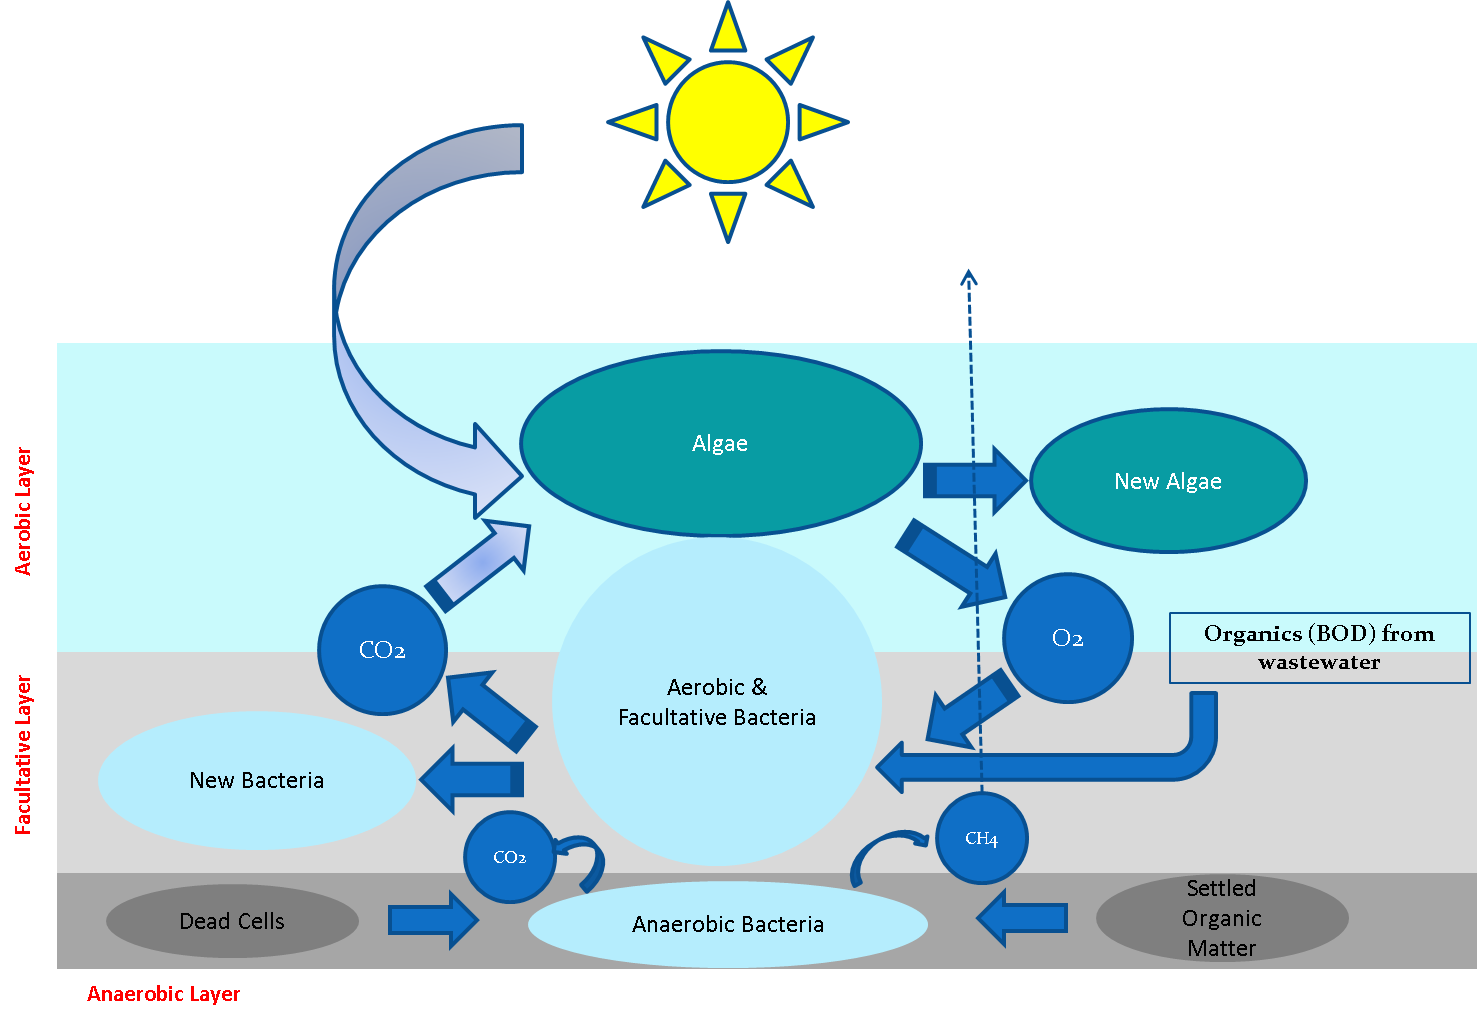
\includegraphics[scale=0.8]{StabilizationPond}\\
Facultative pond schematic
\end{center}
				\end{sidewaysfigure}
				
\subsection{Aerobic Stabilization Ponds}\index{Aerobic Stabilization Ponds}
	
Aerobic stabilization ponds are also known as: \hl{maturation}, \hl{polishing} or \hl{finishing} Pond
\begin{itemize}
\item Typically for tertiary treatment
\item Designed for pathogen removal
\item Shallow - only about 3 feet deep. 
\item They are most often the final cells in a multi-staged pond system
\item They are also used as polishing ponds for tertiary treatment of trickling filter plant effluent.
\item Usually the effluent is directed into a second pond where the sludge can settle 
\item Their shallow depth allows sunlight to penetrate to the bottom of the pond to encourage algae growth and aerobic conditions throughout the pond 
\item The low solids loading found in these tertiary treatment applications means that these ponds normally have no sludge zone
\item These ponds may be mechanically aerated 
\item Aerobic polishing ponds are designed for 15-20 pounds BOD/acre/day
\item Aerobic ponds are typically designed for pathogen removal
\item Aerobic lagoon levels should always maintain at least 18 inches of water in the pond
\end{itemize}



\section{Ponds Operations and Maintenance}\index{Ponds Operations and Maintenance}

\begin{itemize}
\item Ponds and lagoons are designed as continuous discharge, controlled discharge, or no discharge.
\begin{itemize}
\item In controlled discharge ponds the wastewater is held for long periods of time before discharging. 

\item No-discharge ponds the inflow rate needs to be equal or exceed the rates of evaporation and/or percolation. 
\end{itemize}
\item Short-circuiting in a pond may be caused by poor design of inlet and outlet piping arrangements or by uncontrolled growth of water weeds.
\item Stagnant water will breed mosquitoes and can result in anaerobic conditions developing that can cause odor issues 
\item Dikes need to be maintained
\item Aquatic plants and weeds must be removed from the water. 
\item Reeds will create stagnant areas along the edge of the pond and need to be removed
\item To start a new pond, two feet of water is typically added prior to fresh starting wastewater feed. 
\item Sodium nitrate can be used to help recover from an odor-causing upset. The nitrates ($NO_3$) will provide a source of chemically bound oxygen for the bacteria to use instead of dissolved oxygen.
\item Scum control may be required
\end{itemize}

\section{Math Problems}\index{Math Problems}

\subsection{Pond Area}\index{Pond Area}

Formula: \hl{$Pond \enspace Area=Width * Length$}\\
\vspace{0.2cm}
also,     \hl{$Pond \enspace Area=\dfrac{Pond \enspace Volume}{Pond \enspace Depth}$}\\
\vspace{0.2cm}
\hl{Example Problem:}\\
A pond is 260 ft. long and 80 ft. wide. What is the area of this pond in acres?\\ 
\vspace{0.2cm}
Solution:\\
\vspace{0.2cm}
$(260*80)ft^2*\dfrac{acre}{43,560ft^2}=\boxed{0.48acre}$

\subsection{Solids Loading Rate}\index{Solids Loading Rate}


Formula: \hl{$Pond \enspace TSS \enspace loading \enspace rate =  \dfrac{lbs \enspace TSS}{day}$}  \\
\vspace{0.3cm}
\hl{Example Problem:}\\
\vspace{0.3cm}

The influent flow to a pond is 10,000 gallons/hour with a suspended solids concentration of 142mg/L in the raw wastewater.  How many lbs of suspended solids are sent to the pond daily?
\\
Solution:\\
\vspace{0.3cm}
$\dfrac{lbs \enspace TSS}{day}=10,000\dfrac{gal}{hr}*\dfrac{24hrs}{day}*\dfrac{MG}{1,000,000gal}*142\dfrac{mg}{l}*8.34=\boxed{284\dfrac{lbs \enspace TSS}{day}}$

\vspace{0.3cm}

\subsection{Organic Loading Rate}\index{Organic Loading Rate}

\vspace{0.3cm}
Formula: \hl{$Pond \enspace organic \enspace loading \enspace rate =  \dfrac{lbs \enspace BOD/day}{Area (acre)}$}  \\
\vspace{0.3cm}
\hl{Example Problem:}\\
\vspace{0.3cm}
The flow to a pond is 7.2MGD. If the pond diameter is 350 ft and the BOD in the pond influent is 170mg/L, what is the organic loading to this pond in lbs BOD/day/acre?
\\
Solution:\\
\vspace{0.3cm}
$Organic \enspace loading=\dfrac{lbs \enspace BOD \enspace per \enspace day}{area \enspace (acres)}=\dfrac{(7.2MGD \enspace * \enspace 170mg/l \enspace * \enspace 8.34)}{0.785*350^2ft^2}*\dfrac{43,560ft^2}{acre}=\boxed{\dfrac{4,624lbs \enspace BOD}{day-acre}}$

\vspace{0.3cm}

\subsection{Detention time}\index{Detention time}
\vspace{0.3cm}
Formula: \hl{$Pond \enspace detention \enspace time=\dfrac{Volume}{Flow}$}\\ 
\vspace{0.3cm}
\hl{Example Problem:}\\
A 40 acre wastewater treatment pond receives a flow of 0.6 MGD. If the pond is operated at a depth of 4ft. What is the detention time of this pond?\\
Solution:\\
$Pond \enspace detention \enspace time=\dfrac{Volume}{Flow}=\dfrac{(40*4)acre-ft}{0.6*10^6\dfrac{gal}{day}*\dfrac{ft^3}{7.48gal}*\dfrac{acre-ft}{43,560ft^3}}=\boxed{87 \enspace days}$\\
\vspace{0.3cm}


\subsection{Hydraulic Loading Rate}\index{Hydraulic Loading Rate}
Formula:\hl{$Pond \enspace hydraulic \enspace loading \enspace rate \enspace \Bigg[\dfrac{in}{day}\Bigg]=\dfrac{Flow}{Area}$}\\
also, \hl{$Pond \enspace hydraulic \enspace loading \enspace rate \Bigg[\dfrac{in}{day}\Bigg]=\dfrac{Pond \enspace depth \enspace (in)}{Pond \enspace detention  \enspace time \enspace \dfrac{Volume}{Flow}}$ }\\
The second formula above is because:\\
\vspace{0.3cm}
$Hydraulic \enspace Loading \enspace (HL)=\dfrac{Flow}{Area}$\\
\vspace{0.3cm}
$Detention \enspace time \enspace (DT)=\dfrac{Vol}{Flow} \implies Flow=\dfrac{Vol}{DT} $\\
\vspace{0.3cm}
Substituting for flow in  the HL formula above:\\
\vspace{0.3cm}
$HL=\dfrac{\dfrac{Vol}{DT}}{Area}\enspace or \enspace \dfrac{Vol}{Area*DT} \enspace \implies \boxed{HL=\dfrac{Pond \enspace Depth}{DT}} \enspace as \enspace \dfrac{Vol}{Area}=Pond \enspace Depth$\\
\vspace{0.3cm}
\textbf{Example Problems:}\\
\begin{enumerate}

\item Find hydraulic loading in inches/day for a pond given the following:
\begin{itemize}
\item Pond depth = 12ft.
\item Pond volume = 1,400,000ft3
\item Pond flow = 1,000,000gal/day
\end{itemize}
Solution:\\
$Pond \enspace hydraulic \enspace loading \enspace rate \enspace \Bigg[\dfrac{in}{day}\Bigg]=\dfrac{Flow}{Area}$\\
$ \implies\dfrac{1,000,000\dfrac{gal}{day}*\dfrac{ft^3 }{7.48gal}}{\dfrac{1,400,000ft^3}{12ft}}*12\dfrac{in}{ft}=\boxed{13.8\dfrac{in}{day}}$\\
\vspace{0.3cm}
\hl{Note:  The area of the pond was found by dividing the volume (1,000,000$ft^3$) by the pond depth (12ft)}
\vspace{0.3cm}

\item Find pond hydraulic loading in inches/day when the depth of the pond is 6 ft. and the detention time is 30 days.\\
Solution:\\



$Pond \enspace hydraulic \enspace loading \enspace rate=\dfrac{Pond \enspace depth \enspace (in)}{Pond \enspace detention  \enspace time \enspace \dfrac{Volume}{Flow}}$\\
$\implies \dfrac{6*12 \enspace inches}{30 \enspace days}=\boxed{\dfrac{2.4in}{day}}$
\end{enumerate}




\chapterimage{Week5AS.jpg} % Chapter heading image

\chapter{Activated Sludge}


\section{Activated Sludge Basics}\index{Activated Sludge Basics}

Activated sludge is a secondary, biological treatment process used for the removal of suspended and dissolved organic matter from the primary treated wastewater.
\begin{itemize}
\item Utilizes an aeration basin/reactor and a secondary clarifier

\item In the presence of oxygen, aerobic bacteria in the aeration basin consume the organic matter (BOD) in wastewater for their growth and reproduction, converting BOD into bacterial cell mass along with metabolic byproducts including carbon dioxide and water

\item The aerobic bacteria is the predominant microbial life form in the aeration basin.  Other higher microbial life forms — mainly protozoa, are present along with some metazoans.

\item The microorganisms along with their metabolic byproducts and residual dead cell mass form a cluster called floc.

\item The wastewater exiting the aeration basin enters a clarifier where the floc settles.  The clear, treated secondary effluent flows out.

\item A portion of the settled activated sludge floc, is returned from the clarifier to the front of the aeration basin to seed the activated sludge treatment of the incoming primary effluent. The recycled floc is called \textbf{Return Activated Sludge (RAS)}.

\item The remaining settled floc from the clarifier is ”wasted” \textemdash transferred for solids treatment (typically using digestion) prior to its ultimate disposal. The wasted floc is called \textbf{Waste Activated Sludge (WAS)}.

\item The color of healthy activated sludge is tan to brown with an earthy/musty odor.

\begin{center}
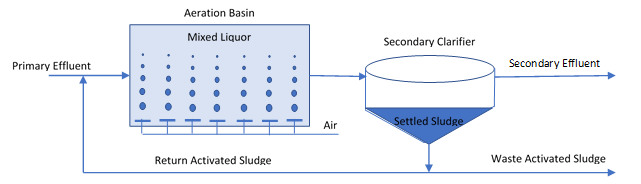
\includegraphics[scale=0.48]{ASProcess}
\end{center}

\item For activated sludge treatment to be effective, it is critical to establish a healthy microbial population which \hl{converts the BOD} into \hl{easily separable biomass.}
\item If the biomass does not settle well in the clarifier, it will be carried out in the treated secondary effluent producing a poor quality effluent with higher solids and organic content.  \\
\end{itemize}

    \begin{mdframed}[backgroundcolor=blue!20] 
\textbf{Mixed liquor}:
\begin{itemize}
\item Mixed liquor is the mixture of raw and/or treated wastewater with the biomass.
\item Mixed liquor sample is typically taken at the end of the aeration reactor.
\item In the mixed liquor, the suspended solids comprised mostly of biomass with some undegraded and non-degradable material is called \textbf{Mixed liquor suspended solids (MLSS)}.  
\item The volatile fraction of the MLSS is termed \textbf{Mixed Liquor Volatile Solids (MLVSS)}.  \item The MLVSS is the amount of biomass as a percentage of the MLSS.  Typically, MLVSS is 70 - 80\%, implying that 70-80\% of the MLSS is volatile (organic) solids.
\end{itemize}
    \end{mdframed}

\section{Activated Sludge Process Control Parameters}\index{Activated Sludge Process Control Parameters}

\subsection{Dissolved Oxygen}\index{Dissolved Oxygen}

Maintaining adequate \textbf{Dissolved oxygen (DO)} is key to the activated sludge process.  DO is typically maintained between 0.5 to 3.0 mg/l in the aeration reactor.\\

\subsection{pH}\index{pH}

The microbiological population in the activated sludge is very sensitive to pH and needs to be maintained at neutral - 7 pH.

\subsection{Temperature}\index{Temperature}

Biological activity is temperature dependent.  Microbial activity approximately doubles for every 10$^o$C rise in temperature.\\

\subsection{Food to Mass Ratio (F:M)}\index{Food to Mass Ratio (F:M)}

In order to establish the amount of the MLSS to be maintained in the aeration tank, the parameter \textbf{Food to Mass Ratio (F:M)} is used.  F:M is the ratio of the "food" – the mass of primary effluent BOD entering the aeration basin to the mass of the microorganisms in the aeration basin \textemdash MLVSS.  Common ranges for F:M for a conventional activated sludge plant are from 0.15 to 0.5\\
\subsection{Sludge Age}\index{Sludge Age}
\begin{itemize}
\item Sludge age is the average time (days) that a sludge particle (cell) spends in the system.  \item Sludge age dictates the presence and predominance of the different types of organisms and is measured as Mean Cell Retention Time (MCRT) or Solids Retention Time (SRT).\\
\item Sludge age is the average time that a sludge particle (cell) spends in the system
\item Conventional AS process - MCRTs are in the range of 5 to 15 days
\item The desired MCRT for a given plant must be found experimentally
\item \hl{F:M and MCRT are inversely related: that is a long MCRT means a low F:M and a short MCRT means a high F:M} 
\item Both, F:M and MCRT values vary from plant to plant and are established through a trial and error process.
\item The MCRT is calculated as:\\ 
\end{itemize}

\vspace{0.2cm}
$MCRT(days) = $\\
$\dfrac{Total \enspace MLSS \enspace lbs \enspace in \enspace the \enspace aeration \enspace system \enspace (aeration \enspace tank \enspace + \enspace clarifier)}{Total \enspace amount \enspace in \enspace lbs/day \enspace of \enspace suspended \enspace solids \enspace leaving  \enspace the \enspace system \enspace(Effluent\enspace SS+ WAS \enspace solids)}$\\
\vspace{0.4cm} 
$MCRT (days) = \dfrac{MLSS \enspace in \enspace aeration \enspace tank \enspace (lbs)+MLSS \enspace in \enspace clarifier \enspace (lbs)}{Effluent \enspace suspended \enspace solids \enspace (lbs/day)+\enspace WAS \enspace SS \enspace (lbs/day)}$\\
\vspace{5mm}
\section{Sludge Settleability}\index{Sludge Settleability}

\begin{itemize}
\item A settleability test is conducted on the mixed liquor from the aeration reactor to  measure the compaction and settleability characteristics of the secondary solids.
\item In the settleability test, a 1-liter mixed liquor sample is allowed to settle for 30-minutes in a graduated cylinder $-$ settleometer. 
\item The \textbf{Sludge Volume Index (SVI)} of the sludge is calculated using results from the 30-minute settleability test and the MLSS value.
\item SVI is expressed in ml/g and it is essentially the volume (ml) of 1 gram of the MLSS after 30 minutes of settling.
\item SVI (ml/g)= $\dfrac{Settled \enspace sludge \enspace volume \enspace in \enspace ml/l \enspace after \enspace 30 \enspace min}{MLSS \enspace mg/l}*1000 \dfrac{mg}{g}$
\item SVI provides a more accurate picture of the sludge settling characteristics than settleability or MLSS alone.
\item 50 to 120 ml/g SVI value is considered optimal.
\item Higher SVI values  indicate sludge that is slow to settle and not compacting well.
\item When SVI values are approaching 200 ml/g, activated sludge process is considered to be "bulking".
\item Regular monitoring of SVI help identify changes occurring in the activated sludge process preventing settling problems before they occur.
\item Like F:M and MCRT, the optimal SVI value for each plant varies and is also established by trial and error.
\end{itemize}
\vspace{5mm}

\section{RAS and WAS Pumping Rates}\index{RAS and WAS Pumping Rates}

The RAS and WAS pumping rates are primarily to control the amount of microbes in the aeration basin and the sludge age.  RAS and WAS adjustments may be necessary to prevent solids build-up in the clarifier which may lead to solids overflowing  with the effluent. Typical RAS flow rates range from 30-100\% of the influent flow rate.

\section{Activated Sludge Microbiology}\index{Activated Sludge Microbiology}

\begin{itemize}
\item In order for it to be effective, the activated sludge process has to sustain complex set of microorganisms which not only effectively remove the organic material from the wastewater in the aeration tank but also settle and compact well in the clarifier to produce a high quality sludge with a low BOD wastewater effluent.
\item Regular microscopic examination of the activated sludge is conducted to assess the composition of the microbial population and diagnose any potential or occurring process issues.  \item As the normal aerobic bacteria present is too small to observe easily, it is the higher microbial forms - mainly the protozoans and metazoans are observed.
\item The floc in an activated sludge has a porous structure and is essentially an aggregate of bacteria and extracelular material including organic polymers - polysaccharides and other substances secreted by the microorganisms, and remnants of dead microorganisms.
\item Typically, the trophic organisms such as the protozoas and rotifers which feed on the bacteria and other particulates are generally present on the outer surface of the flocs.
\item MCRT is the key factor which establishes the organism mix in the activated sludge.  As MCRT increases, the size and complexity of the organisms increases. 
\item The types of organisms predominating in the Mixed Liquor give an indication as to the age of the sludge.
\end{itemize}


\section{Process Issues}\index{Process Issues}

\begin{itemize}
\item Straggler floc:  This condition shows small, light, and fluffy floc particles with poor settling characteristics. It occurs due to young sludge or low MCRT/MLSS levels and may be related to an inadequate microorganism population or an excessive BOD load (high F:M) which causes a log growth situation. The cells become dispersed rather than flocculated, settleability is poor, and the effluent becomes turbid. In this condition oxygen is used up quickly due to the high metabolism rate, and sludge production is high. One tell-tale sign of this condition is the production of huge amounts of a billowing white foam.

\item Pin floc:  Pin floc are larger dimension spherical particles.  When pin floc is present, the sludge settles well in the settleability test but the supernatant is cloudy. This floc consist mostly of floc-forming bacteria without a filament backbone.  This condition occurs at starvation condition when all of the influent BOD has been used up (low F:M) and the old sludge age organisms are now in endogenous respiration.

\item Rising sludge: Under this condition, sludge settles well, compacts on the bottom of the clarifier, then starts to rise in clumps and patches to the surface.  Rising sludge is typically evidenced as brown in color.  Rising sludge occurs due to either denitrification or sludge septicity due to an excessive detention time in the clarifier.  

\item Bulking and Foaming:  Typical bacteria present in activated sludge include spherical, rod shaped and filamentous.  The presence of filamentous bacteria in activated sludge provide the important structural element for the bacterial floc.  However, presence of excessive filametous bacteria results in bulking or foaming.  Bulking is is marked by poor compaction – high SVI - SVI values near or above 200 ml/g.
\item Identifying which filaments are dominating in the system through a microscopic evaluation will help the operator to understand the condition in the treatment system so that corrective changes can be made.\\
\end{itemize}


\section{Math Problems}\index{Math Problems}

\subsection{Mean Cell Residence Time}\index{Mean Cell Residence Time}


The MCRT is calculated as:\\  
\vspace{0.2cm}
$MCRT(days) = $\\
$\dfrac{Total \enspace MLSS \enspace lbs \enspace in \enspace the \enspace aeration \enspace system \enspace (aeration \enspace tank \enspace + \enspace clarifier)}{Total \enspace amount \enspace in \enspace lbs/day \enspace of \enspace suspended \enspace solids \enspace leaving  \enspace the \enspace system \enspace(Effluent\enspace SS+ WAS \enspace solids)}$\\
\vspace{0.4cm} 
$MCRT (days) = \dfrac{MLSS \enspace in \enspace aeration \enspace tank \enspace (lbs)+MLSS \enspace in \enspace clarifier \enspace (lbs)}{Effluent \enspace suspended \enspace solids \enspace (lbs/day)+\enspace WAS \enspace SS \enspace (lbs/day)}$\\
\vspace{0.3cm}
\textbf{Key Points for Solving MCRT Problems}\\
\begin{enumerate}
\item \textbf{MLSS quantification}:\\ 
\begin{itemize}
\item Pounds formula is used to calculate lbs MLSS using: i) aeration tank and the clarifier volumes, and ii) the given MLSS concentration.  
\item The MLSS concentrations for the aeration tank and the clarifier are the same.  So the given MLSS concentration applies to both - the aeration tank and the clarifier
\item Make sure it is the MLSS concentration that you are using not the MLVSS concentration.  
\item If MLSS concentration is not given but instead MLVSS concentration is given, you will need to find the MLSS concentration by dividing the MLVSS conc. by the mixed liquor volatile solids, as MLVSS(conc.) = MLSS * \% volatile solids
\end{itemize}

\item \textbf{Suspended solids quantification}:\\ 
\begin{enumerate}
\item \textbf{Effluent suspended solids}
\begin{itemize}
\item Effluent suspended solids can be quantified using the pounds formula - using the effluent flow (in MGD) and the effluent suspended solids concentration.
\end{itemize}
\item \textbf{WAS suspended solids}
\begin{itemize}
\item Use pounds formula given the WAS flow (make sure it is in MG) and the WAS SS concentration
\item Note that the WAS and RAS streams have the same SS concentration.  If WAS SS concentration is not specified, use the RAS SS concentration
\end{itemize}
\end{enumerate}
\end{enumerate} 

\hl{Example Problems:}\\
\begin{enumerate}
\item In an conventional activated sludge plant  the aeration tank contains 6000 lbs of MLSS and the final clarifier contains 2300 lbs of MLSS. 1450 lbs of solids are wasted each day and 90 lbs/day of solids leave in the final effluent. Calculate the MCRT for this plant.\\
Solution:\\
\vspace{0.2cm} 
$MCRT (days) =  \dfrac{MLSS \enspace in \enspace aeration \enspace tank \enspace (lbs)+MLSS \enspace in \enspace clarifier \enspace (lbs)}{SS \enspace effluent \enspace (lbs/day)+SS \enspace WAS \enspace (lbs/day)}$\\
\vspace{0.2cm} 
$MCRT (days) =  \dfrac{6000lbs \enspace + \enspace 2300 lbs}{90lbs/day\enspace + \enspace 1450 lbs/day}=5.4=\boxed{5days}$\\
\vspace{0.3cm} 
\item A activated sludge plant treats an average influent flow of 4 MGD.  The plant has two  aeration tanks – 0.45 MG volume each and two final clarifiers – 0.2 MG volume each, and a mixed liquor suspended solids concentration averages  1800 mg/l.   The effluent suspended solids concentration averages 18 mg/L. The WAS flow is 100,000 gallons per day has a SS concentration of 6100 mg/L. Calculate the MCRT\\
Solution:\\
$MCRT (days) =  \dfrac{MLSS \enspace in \enspace aeration \enspace tank \enspace (lbs)+MLSS \enspace in \enspace clarifier \enspace (lbs)}{SS \enspace effluent \enspace (lbs/day)+SS \enspace WAS \enspace (lbs/day)}$\\
\vspace{0.3cm} 
$MLSS \enspace in \enspace aeration \enspace tank \enspace (lbs)=2*0.45*1800*8.34=13511lbs$\\
\vspace{0.3cm} 
$MLSS \enspace in \enspace clarifier \enspace (lbs)=2*0.2*1800*8.34=6005lbs$\\
\vspace{0.3cm} 
$SS \enspace effluent \enspace (lbs/day)=4MGD *18mg/l*8.34=600lbs/day$\\
\vspace{0.3cm} 
$SS \enspace WAS \enspace (lbs/day)=\dfrac{100000}{1000000}MGD *4800mg/l*8.34=4003lbs/day$\\
\vspace{0.3cm} 
Plugging in the values calculated above: $MCRT (days) =  \dfrac{13511+6005}{600+4003}=4.2=\boxed{4days}$\\
\end{enumerate}

\subsection{F:M (Food to Microorganism Ratio}\index{F:M (Food to Microorganism Ratio}

\begin{itemize}
\item This parameter ratios the food – the mass of primary effluent BOD entering the aeration basin to the mass of the microorganisms - \textbf{MLVSS}, in the aeration basin.
\item \textbf{Only the mass of the microorganisms (MLVSS) in the aeration basin is used – the mass of microorganisms in the secondary clarifier is not considered}
\item Common ranges for F/M for a conventional activated sludge plant are from 0.15 to 0.5. 
\item The optimum F/M varies from plant to plant and can be determined by trial and error.
\item The F:M may be used to determine the concentration of mixed liquor suspended solids to be maintained in the aeration tank.
\item Generally, low F/M ratios should be carried during the colder months as the microorganism activity (metabolism) is lower.
\item F:M and MCRT are inversely related: that is a long MCRT means a low F:M and a short MCRT means a high F:M
\end{itemize}
F:M=$\dfrac{amount \enspace of \enspace food \enspace coming \enspace in}{amount \enspace of \enspace microorganisms \enspace present}$\\
\vspace{0.3cm}
\hspace{0.7cm}$=\dfrac{(lbs/day) \enspace primary \enspace effluent  \enspace BOD \enspace entering \enspace the  \enspace aeration \enspace tank}{(lbs) \enspace MLVSS \enspace in \enspace the  \enspace aeration \enspace tank}$\\
\vspace{0.3cm}
\textbf{Key Points for Solving F:M Problem}\\
\begin{enumerate}
\item \textbf{Quantifying F:}
\begin{itemize}
\item use the pounds formula to calculate the lbs/day of BOD in the primary effluent.\\
lbs/day BOD = Primary eff. flow (MGD)* Primary eff. BOD concentration (mg/l) * 8.34\\
\end{itemize}
\item \textbf{Quantifying M:}
\begin{itemize}
\item The concentration of the microorganisms is assumed to be the same as the MLVSS concentration
\item \textbf{Only the mass of the microorganisms (MLVSS) in the aeration basin is used – the mass of microorganisms in the secondary clarifier is not considered} 
\item lbs MLVSS may be calculated using pounds formula using the volume of the aeration tank (in MG) and the MLVSS concentration
\item If the MLVSS concentration is not given, it can be calculated from the MLSS and MLSS \% volatile matter (solids) concentration\\
MLVSS = MLSS * \% MLSS volatile solids
\end{itemize}


\hl{Example Problem:}\\
\begin{enumerate}[i.]
\item A conventional activated sludge plant receives an average flow of 5.5 MGD. The influent BOD to the plant averages 230mg/l and the primary effluent BOD average 160 mg/l. The 1 MG aeration tank has an MLSS concentration of 2800 mg/L and the MLVSS volatile solids content is 75\%. Calculated the F:M ratio for this plant.
\vspace{0.3cm}
Solution:\\
\vspace{0.3cm}
F=5.5*160*8.34=7339lbs/day BOD\\
M=1*2800*0.75*8.34=17514lbs MLVSS\\
F:M=$\dfrac{7339}{17514}=\boxed{0.41}$\\

Note:  The 160 mg/l BOD concentration of the primary effluent was used for the F calculation and not 230mg/l - which is the BOD concentration of the flow coming into the plant\\
\end{enumerate}


\subsection{Sludge Volume Index (SVI)}\index{Sludge Volume Index (SVI)}

\begin{itemize}
\item SVI measures the settleability and compactibility of the secondary sludge
\item It is calculated using results from the 30-minute settleability test and the MLSS concentration
\item SVI is expressed in ml/g and it is essentially the volume (ml) of 1 gram of the MLSS after 30 minutes of settling
\item it provides a more accurate picture of the sludge settling characteristics than settleability or MLSS alone
\item 50 to 120 ml/gm SVI value is considered
optimal. Higher SVI values indicate sludge that is slow to settle and not compacting well. When SVI
values are approaching 200 ml/gm, activated sludge process is considered to be "bulking".
\end{itemize}
\end{enumerate}
SVI (ml/g)= $\dfrac{Settled \enspace sludge \enspace volume \enspace in \enspace ml/l \enspace after \enspace 30 \enspace min}{MLSS \enspace mg/l}*1000 \dfrac{mg}{g}$\\
\vspace{0.3cm}
\textbf{Key Points for Solving SVI Problems}\\
\begin{itemize}
\item For the settling test MLSS is typically settled in a 1 liter settleometer.  The volume of the settled solids is therefore read as ml/L.  So if for any reason a larger or smaller volume of the mixed liquor sample is taken, the settle solids value should commensurate with the volume of the MLSS sample.  For example, if a 2 liter settleometer is used and if the solids settle to 400 ml in that settleometer, the ml/L will be 400ml/2L or 200ml/L
\item For some problems, the settled solids volume is provided as a percentage (\%).  So if a 1-liter settlometer is used and the settled solids volume is reported as 25\%, it implies a settled sludge volume of 250ml/L
\end{itemize} 
\hl{Example Problem:}\\
\begin{enumerate}[i.]
\item In an aeration tank, the MLSS is 2500 mg/l and recorded 30-minute settling test indicates 230 ml/L.  What is the sludge volume index?\\
\vspace{0.3cm}
Solution:\\
SVI=$\dfrac{230ml/l}{2500mg/l}*1000\dfrac{mg}{g}=\boxed{92ml/g}$
\end{enumerate}

\chapterimage{QuizIcon.jpg}
\chapter{Week 5 Module Assessment Quiz}



1. Activated sludge is an anaerobic process\\

a. True \\
b. False \\


\vspace{0.3cm}
2. SVI is a measure of the sludge volume that needs to be wasted\\

a. True \\
b. False \\


\vspace{0.3cm}
3. The F in the F to M ratio refers to the pounds of mixed liquor volatile suspended solids under aeration in an activated sludge plant.\\

a. True \\
b. False \\

\vspace{0.3cm}

4. Algae is primarily responsible for the effective working of an anaerobic pond

\vspace{0.3cm}
a. True \\
b. False \\


\vspace{0.3cm}
5. A one acre wastewater treatment pond operated at a depth of 3 feet holds approximately 1 million gallons.\\

a. True \\
b. False \\

\vspace{0.3cm}

6. Facultative ponds are anaerobic on the bottom and aerobic near the surface. \\

a. True \\
b. False \\

\vspace{0.3cm}

7. A 2.5 acre stabilization pond is operated at a depth of five (5) ft. What is the pond detention time if the flow to the pond is 18,000 cu. ft/day?\\

\vspace{0.3cm}
a. 0.02 days \\
b. 6 days\\ 
c. 30.3 days \\
d. 10 days \\

\vspace{0.3cm}

8. A 5 acre stabilization pond is operated at a depth of five (5) ft. What is the pond detention time if the flow to the pond is 30,000 cu. ft/day?\\

\vspace{0.3cm}
a. 0.03 days \\
b. 7.3 days\\ 
c. 36.3 days \\
d. 12 days\\ 

\vspace{0.3cm}

9. Calculate the F to M ratio given the following.\\
Plant flow- 0.8 MGD\\
Aerator vol- 200,000 gal.\\
Clarifier Volume-175,000 gal\\
Primary eff BOD- 120 mg/L\\
MLVSS conc. -1950 mg/L\\


\vspace{0.3cm}


\vspace{0.3cm}
10. At an activated sludge wastewater treatment plant receiving 3.25 MGD, the final effluent suspended solids concentration averages 21.2 mg/L. What would the calculated MCRT value be when the aeration basin carries 2,050 mg/L MLSS and wastes 0.0550 MGD. The waste activated sludge has a concentration of 7,980 mg/L. The aeration tank has a volume of 1.00 MG and the secondary clarifier has an operational volume of 0.250 MG.\\

\vspace{0.3cm}
a. 2.5 days \\
b. 5.0 days\\ 
c. 7.5 days \\
d. 15 days \\
e. 42 days \\

\vspace{1cm}
\textbf{Answers:}\\
1.	b.  \\

\vspace{0.3cm}
2.	b. \\ 


\vspace{0.3cm}
3.	b. \\ 


\vspace{0.3cm}
4.	b.  \\


\vspace{0.3cm}
5.	a. \\ 


\vspace{0.3cm}
6.	a.\\  


\vspace{0.3cm}
7.	c. \\ 
\vspace{0.3cm}
Solution:\\
\vspace{0.3cm}
$Pond \enspace detention \enspace time=\dfrac{Volume}{Flow}=\dfrac{(2.5*5)acre-ft}{18,000\dfrac{ft^3}{day}*\dfrac{acre-ft}{43,560ft^3}}=\boxed{30 \enspace days}$\\ 

\newpage
8.	c.  \\
\vspace{0.3cm}
Solution:\\
$Pond \enspace detention \enspace time=\dfrac{Volume}{Flow}=\dfrac{(5*5)acre-ft}{30,000\dfrac{ft^3}{day}*\dfrac{acre-ft}{43,560ft^3}}=\boxed{36.3 \enspace days}$\\

\vspace{0.3cm}
9.	a.  \\

Solution:\\
\vspace{0.3cm}
$F:M=\dfrac{(lbs/day) \enspace primary \enspace effluent  \enspace BOD \enspace entering \enspace the  \enspace aeration \enspace tank}{(lbs) \enspace MLVSS \enspace in \enspace the  \enspace aeration \enspace tank}$\\
\vspace{0.3cm}
$F:M=\dfrac{120*0.8*8.34}{1950*0.2*8.34}=\boxed{0.25}$\\

\vspace{0.3cm}
10.	b.  \\
\vspace{0.3cm}
Solution:\\
\vspace{0.3cm}
$MCRT (days) =  \dfrac{MLSS \enspace in \enspace aeration \enspace tank \enspace (lbs)+MLSS \enspace in \enspace clarifier \enspace (lbs)}{SS \enspace effluent \enspace (lbs/day)+SS \enspace WAS \enspace (lbs/day)}$\\
\vspace{0.3cm} 
$MLSS \enspace in \enspace aeration \enspace tank \enspace (lbs)=1*2050*8.34=17,097lbs$\\
\vspace{0.3cm} 
$MLSS \enspace in \enspace clarifier \enspace (lbs)=0.25*2050*8.34=4,274.3lbs$\\
\vspace{0.3cm} 
$SS \enspace effluent \enspace (lbs/day)=3.25MGD *21.2mg/l*8.34=574.6 lbs/day$\\
\vspace{0.3cm} 
$SS \enspace WAS \enspace (lbs/day)=0.055MGD *7,980mg/l*8.34=3,660.4lbs/day$\\
\vspace{0.3cm} 
Plugging in the values calculated above: $MCRT (days) =  \dfrac{17,097.6+4,274.3}{574.6+3,660.4}=4.8=\boxed{5 \enspace days}$\\
\vspace{0.2cm}




